
%% bare_conf.tex
%% V1.4b
%% 2015/08/26
%% by Michael Shell
%% See:
%% http://www.michaelshell.org/
%% for current contact information.
%%
%% This is a skeleton file demonstrating the use of IEEEtran.cls
%% (requires IEEEtran.cls version 1.8b or later) with an IEEE
%% conference paper.
%%
%% Support sites:
%% http://www.michaelshell.org/tex/ieeetran/
%% http://www.ctan.org/pkg/ieeetran
%% and
%% http://www.ieee.org/

%%*************************************************************************
%% Legal Notice:
%% This code is offered as-is without any warranty either expressed or
%% implied; without even the implied warranty of MERCHANTABILITY or
%% FITNESS FOR A PARTICULAR PURPOSE!
%% User assumes all risk.
%% In no event shall the IEEE or any contributor to this code be liable for
%% any damages or losses, including, but not limited to, incidental,
%% consequential, or any other damages, resulting from the use or misuse
%% of any information contained here.
%%
%% All comments are the opinions of their respective authors and are not
%% necessarily endorsed by the IEEE.
%%
%% This work is distributed under the LaTeX Project Public License (LPPL)
%% ( http://www.latex-project.org/ ) version 1.3, and may be freely used,
%% distributed and modified. A copy of the LPPL, version 1.3, is included
%% in the base LaTeX documentation of all distributions of LaTeX released
%% 2003/12/01 or later.
%% Retain all contribution notices and credits.
%% ** Modified files should be clearly indicated as such, including  **
%% ** renaming them and changing author support contact information. **
%%*************************************************************************


% *** Authors should verify (and, if needed, correct) their LaTeX system  ***
% *** with the testflow diagnostic prior to trusting their LaTeX platform ***
% *** with production work. The IEEE's font choices and paper sizes can   ***
% *** trigger bugs that do not appear when using other class files.       ***                          ***
% The testflow support page is at:
% http://www.michaelshell.org/tex/testflow/



\documentclass[conference]{IEEEtran}

\usepackage{epsfig}
\usepackage{amssymb}
\usepackage{amsmath}
\usepackage{amsfonts}
\usepackage{algorithm}
\usepackage{algorithmic}
\usepackage{multirow}
\usepackage[font=sf, labelfont={sf,bf}, margin=1cm]{caption}
\usepackage{amsthm}
\usepackage{url}
\newtheorem*{remark}{Remark}


% Some very useful LaTeX packages include:
% (uncomment the ones you want to load)


% *** MISC UTILITY PACKAGES ***
%
%\usepackage{ifpdf}
% Heiko Oberdiek's ifpdf.sty is very useful if you need conditional
% compilation based on whether the output is pdf or dvi.
% usage:
% \ifpdf
%   % pdf code
% \else
%   % dvi code
% \fi
% The latest version of ifpdf.sty can be obtained from:
% http://www.ctan.org/pkg/ifpdf
% Also, note that IEEEtran.cls V1.7 and later provides a builtin
% \ifCLASSINFOpdf conditional that works the same way.
% When switching from latex to pdflatex and vice-versa, the compiler may
% have to be run twice to clear warning/error messages.






% *** CITATION PACKAGES ***
%
%\usepackage{cite}
% cite.sty was written by Donald Arseneau
% V1.6 and later of IEEEtran pre-defines the format of the cite.sty package
% \cite{} output to follow that of the IEEE. Loading the cite package will
% result in citation numbers being automatically sorted and properly
% "compressed/ranged". e.g., [1], [9], [2], [7], [5], [6] without using
% cite.sty will become [1], [2], [5]--[7], [9] using cite.sty. cite.sty's
% \cite will automatically add leading space, if needed. Use cite.sty's
% noadjust option (cite.sty V3.8 and later) if you want to turn this off
% such as if a citation ever needs to be enclosed in parenthesis.
% cite.sty is already installed on most LaTeX systems. Be sure and use
% version 5.0 (2009-03-20) and later if using hyperref.sty.
% The latest version can be obtained at:
% http://www.ctan.org/pkg/cite
% The documentation is contained in the cite.sty file itself.






% *** GRAPHICS RELATED PACKAGES ***
%
\ifCLASSINFOpdf
  % \usepackage[pdftex]{graphicx}
  % declare the path(s) where your graphic files are
  % \graphicspath{{../pdf/}{../jpeg/}}
  % and their extensions so you won't have to specify these with
  % every instance of \includegraphics
  % \DeclareGraphicsExtensions{.pdf,.jpeg,.png}
\else
  % or other class option (dvipsone, dvipdf, if not using dvips). graphicx
  % will default to the driver specified in the system graphics.cfg if no
  % driver is specified.
  % \usepackage[dvips]{graphicx}
  % declare the path(s) where your graphic files are
  % \graphicspath{{../eps/}}
  % and their extensions so you won't have to specify these with
  % every instance of \includegraphics
  % \DeclareGraphicsExtensions{.eps}
\fi
% graphicx was written by David Carlisle and Sebastian Rahtz. It is
% required if you want graphics, photos, etc. graphicx.sty is already
% installed on most LaTeX systems. The latest version and documentation
% can be obtained at:
% http://www.ctan.org/pkg/graphicx
% Another good source of documentation is "Using Imported Graphics in
% LaTeX2e" by Keith Reckdahl which can be found at:
% http://www.ctan.org/pkg/epslatex
%
% latex, and pdflatex in dvi mode, support graphics in encapsulated
% postscript (.eps) format. pdflatex in pdf mode supports graphics
% in .pdf, .jpeg, .png and .mps (metapost) formats. Users should ensure
% that all non-photo figures use a vector format (.eps, .pdf, .mps) and
% not a bitmapped formats (.jpeg, .png). The IEEE frowns on bitmapped formats
% which can result in "jaggedy"/blurry rendering of lines and letters as
% well as large increases in file sizes.
%
% You can find documentation about the pdfTeX application at:
% http://www.tug.org/applications/pdftex





% *** MATH PACKAGES ***
%
%\usepackage{amsmath}
% A popular package from the American Mathematical Society that provides
% many useful and powerful commands for dealing with mathematics.
%
% Note that the amsmath package sets \interdisplaylinepenalty to 10000
% thus preventing page breaks from occurring within multiline equations. Use:
%\interdisplaylinepenalty=2500
% after loading amsmath to restore such page breaks as IEEEtran.cls normally
% does. amsmath.sty is already installed on most LaTeX systems. The latest
% version and documentation can be obtained at:
% http://www.ctan.org/pkg/amsmath





% *** SPECIALIZED LIST PACKAGES ***
%
%\usepackage{algorithmic}
% algorithmic.sty was written by Peter Williams and Rogerio Brito.
% This package provides an algorithmic environment fo describing algorithms.
% You can use the algorithmic environment in-text or within a figure
% environment to provide for a floating algorithm. Do NOT use the algorithm
% floating environment provided by algorithm.sty (by the same authors) or
% algorithm2e.sty (by Christophe Fiorio) as the IEEE does not use dedicated
% algorithm float types and packages that provide these will not provide
% correct IEEE style captions. The latest version and documentation of
% algorithmic.sty can be obtained at:
% http://www.ctan.org/pkg/algorithms
% Also of interest may be the (relatively newer and more customizable)
% algorithmicx.sty package by Szasz Janos:
% http://www.ctan.org/pkg/algorithmicx




% *** ALIGNMENT PACKAGES ***
%
%\usepackage{array}
% Frank Mittelbach's and David Carlisle's array.sty patches and improves
% the standard LaTeX2e array and tabular environments to provide better
% appearance and additional user controls. As the default LaTeX2e table
% generation code is lacking to the point of almost being broken with
% respect to the quality of the end results, all users are strongly
% advised to use an enhanced (at the very least that provided by array.sty)
% set of table tools. array.sty is already installed on most systems. The
% latest version and documentation can be obtained at:
% http://www.ctan.org/pkg/array


% IEEEtran contains the IEEEeqnarray family of commands that can be used to
% generate multiline equations as well as matrices, tables, etc., of high
% quality.




% *** SUBFIGURE PACKAGES ***
%\ifCLASSOPTIONcompsoc
%  \usepackage[caption=false,font=normalsize,labelfont=sf,textfont=sf]{subfig}
%\else
%  \usepackage[caption=false,font=footnotesize]{subfig}
%\fi
% subfig.sty, written by Steven Douglas Cochran, is the modern replacement
% for subfigure.sty, the latter of which is no longer maintained and is
% incompatible with some LaTeX packages including fixltx2e. However,
% subfig.sty requires and automatically loads Axel Sommerfeldt's caption.sty
% which will override IEEEtran.cls' handling of captions and this will result
% in non-IEEE style figure/table captions. To prevent this problem, be sure
% and invoke subfig.sty's "caption=false" package option (available since
% subfig.sty version 1.3, 2005/06/28) as this is will preserve IEEEtran.cls
% handling of captions.
% Note that the Computer Society format requires a larger sans serif font
% than the serif footnote size font used in traditional IEEE formatting
% and thus the need to invoke different subfig.sty package options depending
% on whether compsoc mode has been enabled.
%
% The latest version and documentation of subfig.sty can be obtained at:
% http://www.ctan.org/pkg/subfig




% *** FLOAT PACKAGES ***
%
%\usepackage{fixltx2e}
% fixltx2e, the successor to the earlier fix2col.sty, was written by
% Frank Mittelbach and David Carlisle. This package corrects a few problems
% in the LaTeX2e kernel, the most notable of which is that in current
% LaTeX2e releases, the ordering of single and double column floats is not
% guaranteed to be preserved. Thus, an unpatched LaTeX2e can allow a
% single column figure to be placed prior to an earlier double column
% figure.
% Be aware that LaTeX2e kernels dated 2015 and later have fixltx2e.sty's
% corrections already built into the system in which case a warning will
% be issued if an attempt is made to load fixltx2e.sty as it is no longer
% needed.
% The latest version and documentation can be found at:
% http://www.ctan.org/pkg/fixltx2e


%\usepackage{stfloats}
% stfloats.sty was written by Sigitas Tolusis. This package gives LaTeX2e
% the ability to do double column floats at the bottom of the page as well
% as the top. (e.g., "\begin{figure*}[!b]" is not normally possible in
% LaTeX2e). It also provides a command:
%\fnbelowfloat
% to enable the placement of footnotes below bottom floats (the standard
% LaTeX2e kernel puts them above bottom floats). This is an invasive package
% which rewrites many portions of the LaTeX2e float routines. It may not work
% with other packages that modify the LaTeX2e float routines. The latest
% version and documentation can be obtained at:
% http://www.ctan.org/pkg/stfloats
% Do not use the stfloats baselinefloat ability as the IEEE does not allow
% \baselineskip to stretch. Authors submitting work to the IEEE should note
% that the IEEE rarely uses double column equations and that authors should try
% to avoid such use. Do not be tempted to use the cuted.sty or midfloat.sty
% packages (also by Sigitas Tolusis) as the IEEE does not format its papers in
% such ways.
% Do not attempt to use stfloats with fixltx2e as they are incompatible.
% Instead, use Morten Hogholm'a dblfloatfix which combines the features
% of both fixltx2e and stfloats:
%
% \usepackage{dblfloatfix}
% The latest version can be found at:
% http://www.ctan.org/pkg/dblfloatfix




% *** PDF, URL AND HYPERLINK PACKAGES ***
%
%\usepackage{url}
% url.sty was written by Donald Arseneau. It provides better support for
% handling and breaking URLs. url.sty is already installed on most LaTeX
% systems. The latest version and documentation can be obtained at:
% http://www.ctan.org/pkg/url
% Basically, \url{my_url_here}.




% *** Do not adjust lengths that control margins, column widths, etc. ***
% *** Do not use packages that alter fonts (such as pslatex).         ***
% There should be no need to do such things with IEEEtran.cls V1.6 and later.
% (Unless specifically asked to do so by the journal or conference you plan
% to submit to, of course. )


% correct bad hyphenation here
\hyphenation{op-tical net-works semi-conduc-tor}
\usepackage{graphicx}
\usepackage{amssymb}
\usepackage{amsmath}
\usepackage{amsfonts}
\usepackage{algorithm}
\usepackage{algorithmic}
\usepackage{subfigure}

\begin{document}
%
% paper title
% Titles are generally capitalized except for words such as a, an, and, as,
% at, but, by, for, in, nor, of, on, or, the, to and up, which are usually
% not capitalized unless they are the first or last word of the title.
% Linebreaks \\ can be used within to get better formatting as desired.
% Do not put math or special symbols in the title.
\title{A Probabilistic View of Neighborhood-based Recommendation Methods}


% author names and affiliations
% use a multiple column layout for up to three different
% affiliations
\author{\IEEEauthorblockN{Jun Wang}
\IEEEauthorblockA{ University of Luxembourg \\
jun.wang@uni.lu}
\and
\IEEEauthorblockN{Qiang Tang}
\IEEEauthorblockA{ University of Luxembourg\\
tonyrhul@gmail.com}}


% make the title area
\maketitle
\begin{abstract}
Probabilistic graphic model is an elegant framework to compactly present complex real-world observations by modeling uncertainty and logical flow (conditionally independent factors). In this paper, we present a probabilistic framework of neighborhood-based recommendation methods (PNBM) in which \emph{similarity} is regarded as an unobserved factor. Thus, PNBM leads the estimation of user preference to maximizing a  posterior over \emph{similarity}. We further introduce a novel multi-layer \emph{similarity} descriptor which models and learns the joint influence of various features under PNBM, and name the new framework MPNBM. Empirical results on real-world datasets show that MPNBM allows very accurate estimation of user preferences.
\end{abstract}

\section{Introduction}
\label{introduction}
%With the rapid growth of online markets, recommender systems have been extensively deployed to provide friendly user experience and increase business income.
Collaborative filtering, which leverages user history information to predict users' unknown preference, is one of the most successful techniques to build recommender systems \cite{su2009survey}. Matrix factorization (MF) \cite{koren2009matrix} and neighborhood-based methods (NBMs) \cite{desrosiers2011comprehensive} are two representative approaches. MF family attracts more attention due to its ability of modeling influence of various features (e.g. \cite{zheng2015incorporating, yang2016learning, koren2008factorization}), thus to improve accuracy. However, it is difficult to provide explainable recommendation results. NBM family, shown as Fig. \ref{strnbm}, is very popular mainly due to the fact that it naturally explains recommendation results (e.g. An item which is similar with what you bought before). \emph{Similarity} serves as the basis of weighting neighbors which is crucial to the accuracy of NBM recommender systems. However, existing \emph{similarity} computation scheme is incapable of capturing influence from different features which hampers further polishing \emph{similarity} to improve accuracy. In this paper, we first present a basic probabilistic framework of NBM family (PNBM) which leads learning \emph{similarity} to a regression problem. Then we introduce a novel multi-layer \emph{similarity} descriptor which models and learns the joint influence of different features under PNBM.


\subsection{Related Work}
\label{relwork1}
Commonly, NBMs are divided into two classes \cite{desrosiers2011comprehensive}. One is user-based approach which predicts the rating that a user will assign to an unrated item by referring to other users who are similar to this user. The other is item-based approach which estimates a user's preference to an unrated item based on other items that are similar to this unrated item. The two approaches follow the same principle.
% In the rest of this paper, we use item-based approach as an example, and our discussions can be applied to the user-based approach in a straightforward manner.

With respect to NBM, researches have mainly focused on \emph{similarity} computation schemes \cite{desrosiers2011comprehensive} and neighbor selection strategies \cite{adamopoulos2014over}.  \emph{Similarity} also serves as the basis for neighbor selection, thus we concentrate upon \emph{similarity} in this paper. Generally, there are two main approaches to compute \emph{similarity}. One introduces different kinds of correlation coefficients as \emph{similarity} \cite{desrosiers2011comprehensive}, such as Pearson and Cosine correlations. However, some researchers argue that such kind of methods isolate the relations between two items without leveraging global information. The other approach learns \emph{similarity} via regression models. \cite{bell2007scalable, toscher2008improved} introduce a way to learn similarity by minimizing mean squared error between observed ratings and their corresponding estimation. \cite{toscher2008improved} factors similarity matrix via low-rank approximations. \cite{bell2007modeling} presents a weighted  error function which gives more weight to the users who rated items most similar to the estimated item.  \cite{ning2011slim,rendle2009bpr} simplify standard neighborhood-based models to a simple linear regression problem for top-$N$ recommendation based on binary databases.

\begin{figure}[t]
\centering
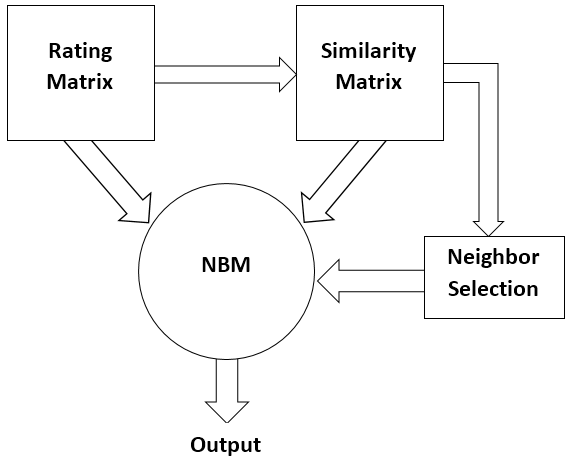
\includegraphics[height=2.0in, width=2.4in]{nmb1}
\caption{ A general structure of NBM}
\label{strnbm}
\end{figure}

A number of probabilistic models have been introduced to collaborative filtering. However, only a very small portion of them are NBM related.
%most of which are for MF( e.g. \cite{mnih2007probabilistic} \cite{salakhutdinov2008bayesian} \cite{ahn2015large}).
 \cite{rendle2009bpr} presents a generic Bayesian personalized ranking framework which is optimized for the area under ROC (AUC) metric. \cite{yu2004probabilistic} introduces a probabilistic memory-based collaborative filtering method in which they use a mixture Gaussian model built on the basis of a set of user profiles and use the posterior distribution of user ratings for prediction.  \cite{defazio2012graphical} builds a Markov network using Pearson-correlation NBM as basis. People also place probabilistic prior assumptions to observations to model uncertainty. Such as, \cite{guo2013novel} places Dirichlet distribution on the absolute value of rating difference. \cite{adamopoulos2014over} uses different probabilistic density functions to sample neighbors from a predefined similarity matrix (vectors).

Unfortunately, these models are incapable of representing complex features, and none of them discusses NBM family itself from a Bayesian perspective.
\subsection{Contribution}

In this paper, we present a probabilistic (Bayesian) framework of NBM family, and our contribution is twofold.

\begin{itemize}
\item First, we present a general graphical model of NBM family (PNBM) which leads the estimation of user preference to maximizing a posterior over \emph{similarity}.
\item Then, we introduce a novel multi-layer \emph{similarity} descriptor which  is capable of modeling and learning the joint influence of various features (e.g. rating, text, genre) under PNBM, and we name the new framework as MPNBM.
\end{itemize}

MPNBM is evaluated on three popular real-world datasets via root-mean-square-error (RMSE) metric. Empirical results show that MPNBM consistently outperform state-of-art approaches  on the datasets we choose.

\section{Preliminary}
\label{preliminary}
Suppose we have a data set organized in form of $User \times Item$ matrix $R \in \mathbb{R}^{N\times M}$, it contains $N$ users and $M$ items. $S \in \mathbb{R}^{M\times M}$ is item \emph{similarity} matrix, $s_{ij}$ denotes similarity between item $i$ and $j$, we further assume $s_{ij}=s_{ji}$. $I \in \mathbb{B}^{N\times M}$ presents indicator matrix, and $ \mathbb{B} =  \{ 0,1\}$. $I_{ui}=1$ if user $u$ rated item $i$, otherwise $I_{ui}=0$. $R^{>0} \subset  R $ denotes all the observed ratings.

So far, many neighborhood-based methods have been proposed, as surveyed in \cite{desrosiers2011comprehensive}. For simplicity, we take a variant of mean-centering NBM \cite{resnick1994grouplens} as instance throughout the paper. The predication formula is defined in Equation (\ref{myeq:mc}).
\begin{equation}\label{myeq:mc}
 \hat{r}_{ui}' = \bar{r}_{i} + \frac{\sum_{j\in \mathcal{I} \backslash \{i\}}s_{ij}(r'_{uj}-\bar{r}_j)I_{uj}}{\sum_{j \in \mathcal{I} \backslash \{i\}}|s_{ij}|I_{uj}}
\end{equation}
where  $r'_{uj}$ is rating score that user $u$ gave to item $j$. $\hat{r}_{ui}'$ denotes the estimation of user $u$'s preference on item $i$. $\bar{r}_i$ is the mean value of all the ratings given to item $i$. $\mathcal{I}$ presents a set containing all the items.

%$j\in \mathcal{I} \backslash i$ denotes any item $j$ in $\mathcal{I}$ except item $i$.

For further simplicity,
%we abuse the notation a bit, by letting $r_{ui}=(r_{ui}-\bar{r}_i)I_{ui}$. Then
Equation (\ref{myeq:mc}) is transformed into a vectorization form:
\begin{equation}\label{myeq:basic}
\hat{r}_{ui} = \frac{\sum_{j\in \mathcal{I} \backslash \{i\}}s_{ij}r_{uj}}{\sum_{j \in \mathcal{I} \backslash \{i\}}|s_{ij}|I_{uj}}=\frac{S_iR_u^{-}}{|S_i|I_u^{-}}
\end{equation}
where $\hat{r}_{ui} = \hat{r}_{ui}'-\bar{r}_{i}$ and $r_{ui}=(r'_{ui}-\bar{r}_i)I_{ui}$.  $S_{i} \in \mathbb{R}^{1\times M}$ denotes \emph{similarity} vector corresponding to item $i$ and  $R_{u} \in \mathbb{R}^{N\times 1}$ represents rating vector of user $u$. The multiplication $S_{i}R_{u}$ denotes the inner product of the two vectors. $I_{u} \in \mathbb{B}^{N\times 1}$ is an indicator vector of user $u$. The symbol $\cdot ^-$ means a vector that does not contain an item which is being predicted. For example, with regard to Equation (\ref{myeq:basic}), $R_{u}^-$ denotes a vector does not contain $r_{ui}$.  Moreover, we assume the testing set is excluded from the training set, when we predict $\hat{r}_{ui}$ in the testing set, $r_{ui}$ in the training set is always zero.

\section{Probabilistic Framework of NBM}
\label{asimple}

\begin{figure}[ht!]
\centering
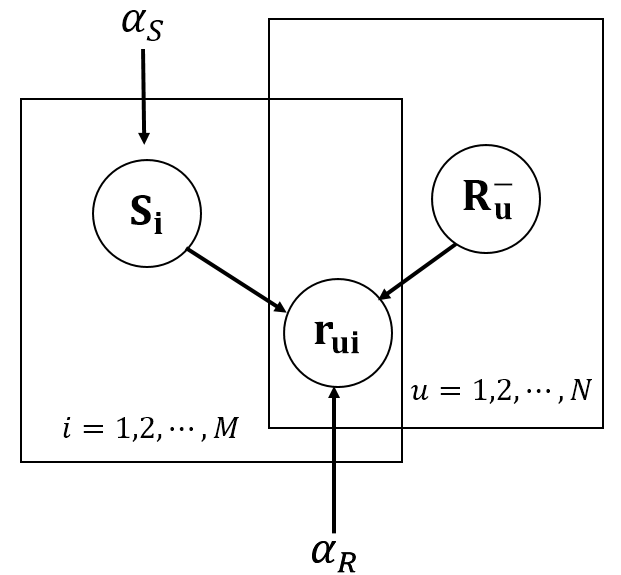
\includegraphics[height=2.3in, width=2.4in]{graph-pnbm}
\caption{Graphical model of PNBM}
\label{gpnbm}
\end{figure}

In this section, we present a probabilistic graphical model of NBMs (PNBM), shown in Fig. \ref{gpnbm}. It is a Bayesian network which describes the following factorization:

\begin{equation}\label{myeq:pnbm}
\begin{split}
p(S_i, R_u^{-}, & r_{ui}, \alpha_S, \alpha_R) = \\ & p(R_u^{-})p(\alpha_S)p(\alpha_R)p(r_{ui}|S_i,R_u^{-},\alpha_R)p(S_i|\alpha_S)
\end{split}
\end{equation}

In our context, placing prior distribution on hyper-parameters $\Theta \{ \alpha_S, \alpha_R \}$ does not significantly improve accuracy while dramatically increasing time complexity. For the sake of simplicity and reduction of time complexity, we simply  let $p(\alpha_S), \ p(\alpha_R)$ be constant, and $p(R_u^{-})$ is also constant. So we can simplify Equation (\ref{myeq:pnbm}) to

\begin{equation}\label{myeq:pnbm2}
p(S_i, R_u^{-},  r_{ui}, \alpha_S, \alpha_R) \propto  p(r_{ui}|S_i,R_u^{-},\alpha_R)p(S_i|\alpha_S)
\end{equation}

% It is inspired by \cite{dueck2004probabilistic, mnih2007probabilistic}, while they focus on matrix factorization.

We introduce a general Gaussian distribution (but not limited to, other distribution can be also applied to. It depends on real-world context.) to density function $p(*)$ which naturally leads to a sum-of-square-error.

More specifically, assume that an item's similarity vector $S_i$ is independent from those of other items, and $S_i$ is sampled from a mean-zero spherical Gaussian distribution. Thus we have
\begin{equation}\label{myeq:gsim}
p(S|\alpha_{S})=\prod_{i=1}^{M} \mathcal{N}(S_{i}|0, \alpha_{S}^{-1}\mathbf{I})
\end{equation}
where $\mathcal{N}(x|\mu,\alpha^{-1})$ denotes the Gaussian distribution for $x$ with mean $\mu$ and precision $\alpha$.
We also assume that ratings are independent with each other. Combine with Equation (\ref{myeq:basic}), we have following
 \begin{equation}\label{myeq:grate}
p(R^{>0}|S,R^-,\alpha_{R}) = \prod_{i=1}^{M}\prod_{u=1}^{N}[\mathcal{N}(r_{ui}|\frac{S_{i}R_{u}^-}{|S_{i}|I_{u}^-}, \alpha_{R}^{-1}) ]^{I_{ui}}
\end{equation}

\section{Multi-layer \emph{Similarity} Descriptor}
\label{cpnbm}
In Section \ref{asimple}, we introduced a general probabilistic (Bayesian) NBM framework which is simple and straightforward. However, like other similarity computation methods, PNBM falls short in  feature representation which extremely limits the accuracy improvement.  In this section, we present a multi-layer \emph{similarity} descriptor (MLSD, shown in Fig.\ref{g:mlsd} ) which is able to model and learn the joint influence of various features (e.g. ratings, text, genre, time). MLSD is mathematically defined as

\begin{figure}[t]
\centering
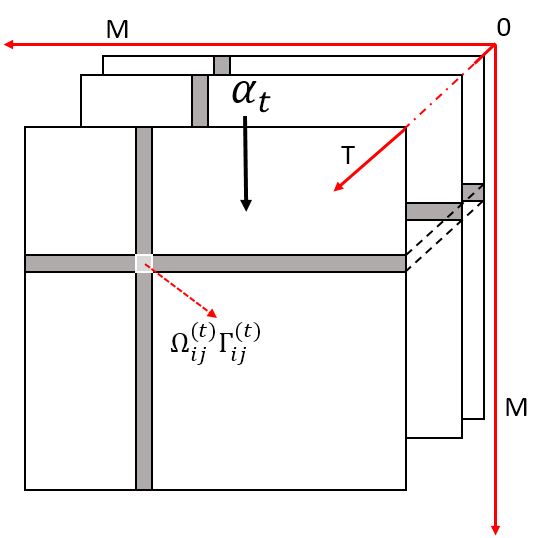
\includegraphics[height=2.0in, width=2.4in]{mlsd}
\caption{Multi-layer \emph{similarity} descriptor. Each layer models an influence generated from features. }
\label{g:mlsd}
\end{figure}

\begin{equation}\label{myeq:geneconstrainsim}
 \mathcal{S} =\sum_{t=1}^{T}\phi^{(t)}(\Omega^{(t)} \circ \Gamma^{(t)})
\end{equation}
where $\Gamma^{(t)}\in \mathbb{R}^{M\times M}$ denotes the \emph{similarity} basis at $t$-th layer. $\Omega^{(t)} \in \mathbb{R}^{M\times M}$ is $\Gamma^{(t)}$'s constraint matrix which presents an influence of observed features.  For example, it can present the similarity of text description ( or time closeness ) between any two-item. Note that different influences may be generated from the same feature. $\phi^{(t)}$ denotes the importance of the feature-influence modeled at layer $t$. $T$ is the number of layers (influence) employed to model \emph{similarity}. In this paper, we don't require $\sum_{t=1}^{T}\phi^{(t)}=1$, since we always have a normalization factor $|S_i|I_u^-$ in the prediction equation, i.e. Equation (\ref{myeq:basic}). $A \circ B$ denotes point-wise product operation (Hadamard product) on matrices $A$ and $B$, e.g.
$$\begin{pmatrix}
a_{11} &  a_{12}\\
a_{21} &  a_{22}
\end{pmatrix} \circ
\begin{pmatrix}
b_{11} &  b_{12}\\
b_{21} &  b_{22}
\end{pmatrix} =
\begin{pmatrix}
a_{11}b_{11} &  a_{12}b_{12}\\
a_{21}b_{11}&  a_{22}b_{22}
\end{pmatrix} $$

MLSD can be smoothly integrated into PNBM, shown in Fig. \ref{g:mpnbm}, named MPNBM. The Bayesian network is mathematically describe as
\begin{equation}\label{myeq:mpnbm}
\begin{split}
p(R_u^{-}, &  r_{ui}, \Gamma^{(t)}_{i}, \Omega^{(t)}_{i}, \alpha_t, \alpha_R) \propto \\
& p(r_{ui}|S_i,R_u^{-},\alpha_R)\prod_{t=1}^{T}  p(\Omega^{(t)}_{i} \circ \Gamma^{(t)}_{i} |\alpha_t)
\end{split}
\end{equation}
where $ \mathcal{S}_i =\sum_{t=1}^{T}\phi^{(t)}(\Omega^{(t)}_i \circ \Gamma^{(t)}_i)$.
Follow the same assumptions in Section \ref{asimple}, we define the prior of layer $t$   ( $\Omega^{(t)}_i \circ \Gamma^{(t)}$) as
\begin{equation}\label{myeq:mulsim}
 p(\Omega^{(t)} \circ \Gamma^{(t)}|\alpha_{t})=\prod_{i=1}^{M} \mathcal{N}(\Omega^{(t)}_{i} \circ \Gamma^{(t)}_{i}|0, \alpha_{t}^{-1}\mathbf{I})
\end{equation}
And we have the conditional distribution over observed ratings defined as
\begin{equation}\label{myeq:rmul}
\begin{split}
p(R^{>0}| & \Omega^{(t)},  \Gamma^{(t)}, R^-, \alpha_R) = \\
& \prod_{i=1}^{M}\prod_{u=1}^{N}\mathcal{N}[(r_{ui}|\frac{(\sum_{t=1}^{T}\phi^{(t)}\Omega^{(t)} \circ \Gamma^{(t)})R_u^{-}}{(\sum_{t=1}^{T}\phi^{(t)}\Omega^{(t)} \circ \Gamma^{(t)})I_u^{-}}, \alpha_R^{-1})]^{I_{ui}}
\end{split}
\end{equation}
\begin{figure}[t]
\centering
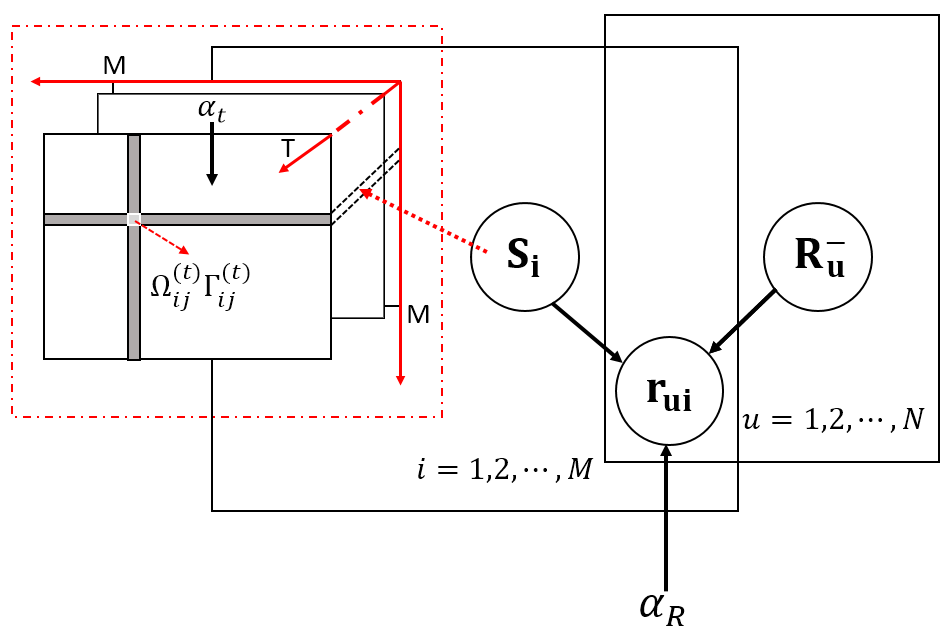
\includegraphics[height=2.2in, width=3.25in]{mpnbm}
\caption{Graphical model of MPNBM.  Note that only black solid arrows ($\rightarrow$) denote the dependency flow in the graphical model.}
\label{g:mpnbm}
\end{figure}

\section{Maximum a Posterior}
\label{map-1}
PNBM is a specific case of MPNBM, which only has one layer with constraint-matrix set to 1. In this section, we take MPNBM as example to present how we optimize \emph{similarity} via maximizing a posterior.

The log of Bayesian network defined in Equation (\ref{myeq:mpnbm}) is given by
\begin{equation}\label{myeq:logmpnbm}
\begin{split}
\log p( & R_u^{-}, r_{ui}, \Gamma^{(t)}_{i}, \Omega^{(t)}_{i}, \alpha_t, \alpha_R) \propto \\
& \log p(r_{ui}|S_i,R_u^{-},\alpha_R) + \sum_{t=1}^{T}  p(\Omega^{(t)}_{i} \circ \Gamma^{(t)}_{i} |\alpha_t)
\end{split}
\end{equation}

In fact, it defines the posterior distribution over \emph{similarity}.
Combine it with Equation (\ref{myeq:mulsim}) and Equation (\ref{myeq:rmul}), we have

\begin{equation}\label{myeq:logmpnbm2}
\begin{split}
-  \log &  p(R^{-}, R, \Gamma^{(t)}_{i}, \Omega^{(t)}_{i}, \alpha_t, \alpha_R) \propto \\
& \frac{\alpha_R}{2} \sum_{i=1}^M\sum_{u=1}^N(r_{ui}-\frac{S_iR_u^-}{|S_i|I_u^-})^2+\frac{\alpha_t}{2}\sum_{t=1}^{T}\sum_{i=1}^M(||\Omega^{(t)}_{i} \circ \Gamma^{(t)}_{i}||_2)\\
+& M^2 \sum_{i=1}^T\log \frac{\alpha_t}{\sqrt{2\pi}} + \log \frac{\alpha_R}{\sqrt{2\pi}} \sum_{i=1}^M\sum_{u=1}^NI_{ui}
\end{split}
\end{equation}

Maximizing the above Bayesian network distribution with hyper-parameters being kept fixed is equivalent to minimizing an error function defined as

\begin{equation}\label{myeq:errfunc}
\mathcal{E} = \frac{1}{2} \sum_{i=1}^M\sum_{u=1}^N(r_{ui}-\frac{S_iR_u^-}{|S_i|I_u^-})^2+\sum_{t=1}^{T}\sum_{i=1}^M(\lambda_t ||\Omega^{(t)}_{i} \circ \Gamma^{(t)}_{i}||_2)
\end{equation}
where $\lambda_t = \frac{\alpha_t}{2\alpha_R}$ is the regularization parameter for layer $t$.

A simple linear Gaussian model sometimes makes prediction value fall out of the range of valid rating values. In order to force the predication values to fall into valid range, we pass the linear-Gaussian model through hyperbolic tangent function $h(x)= \frac{e^x-e^{-x}}{e^x+e^{-x}}$
which makes prediction values be in range of [-1,1].
We map the centralized ratings to range [-1, 1] with Equation (\ref{myeq:mapf}).
\begin{equation}\label{myeq:mapf}
t(x)= \frac{x-\frac{max_x+min_x}{2}}{max_x-\frac{max_x+min_x}{2}}
\end{equation}
where $max_x$ and $min_x$ are the max and min value of ratings, respectively. Since the ratings are centralized by their corresponding mean value, we always have $max_x>0$ and $min_x<0$. As a result, the range of valid rating value align with the estimation produced by our models.

The conditional distribution of observed ratings  becomes
%\begin{small}
\begin{equation}\label{myeq:gratetanh}
p(R^{>0}|S,R^-,\alpha_{R}) = \prod_{i=1}^{M}\prod_{u=1}^{N}[\mathcal{N}(r_{ui}|h(\frac{S_{i}R_{u}^-}{|S_{i}|I_{u}^-}), \alpha_{R}^{-1}) ]^{I_{ui}}
\end{equation}
%\end{small}

We adopt stochastic gradient descent (SGD) as learning algorithm to train latent factors, shown in Algorithm \ref{alg:sgd}.

\begin{algorithm}[h]
   \caption{Training via Stochastic Gradient Descent}
   \label{alg:sgd}
\begin{algorithmic}
   \STATE {\bfseries Preliminary:} rating matrix $R$, error function.
   \STATE {\bfseries Initialization:} similarity basis $\Gamma^{(t)}$, influence constraint-matrix $\Omega^{(t)}$, influence importance factor $\phi^{(t)}$, learning rate $\beta$, regular parameter $\lambda_{t}$. Note that $ \mathcal{S}_i =\sum_{t=1}^{T}\phi^{(t)}(\Omega^{(t)}_i \circ \Gamma^{(t)}_i)$.
   \STATE $\bullet \ \ $ Training:
   \FOR{$k=1$ {\bfseries to} $K$}
   \STATE $\bullet \ \ $ For each layer ($t$), point-wisely update the similarity basis $\Gamma^{(t)}_{ij}$:
   \STATE $\quad \quad [\Gamma_{ij}^{(t)}]^{new} =[\Gamma_{ij}^{(t)}]^{old}-\beta  e_{ui} \frac{\partial \hat{r}_{ui} }{\partial \Gamma^{(t)} _{ij}}-\beta \lambda_{t}(\Omega^{(t)}_{ij} \circ \Gamma^{(t)}_{ij})$
   \STATE $\bullet \ \ $ where $e_{ui}=\hat{r}_{ui}-r_{ui}$.
   \ENDFOR
   \STATE {\bfseries Prediction:} prediction using Equation (\ref{myeq:mc}) with top-$200$ the most similar neighbors.
\end{algorithmic}
\end{algorithm}

\section{Experiments}

\label{experiments}
\subsection{Description of Data Sets}
In the experiments, we evaluate our models and state-of-art methods over three different data sets, summarized in Table \ref{dataset-table}.

\begin{table}[h!]
\centering
\caption{Data Sets}
\hspace*{-0.3cm}
\begin{tabular}{|c|c|c|c|c|l|} \hline
data set & user\# & item\# & ratings\# &scales & density \\ \hline
ML-20M  & 138,493 & 26,744 &20,000,263&[0.5,5] & 0.54\%\\ \hline
ML-10M  & 69,878 & 1,0677 &10,000,054&[0.5,5] & 1.34\%\\ \hline
Netflix & 32,682 & 13,139 &3,967,477&[1,5] & 0.92\% \\
\hline
Yahoo-R4 & 7,637& 3,791&207,854&[1,5] & 0.72\%\\
%ML-1M & 6,040 & 3,952&1,000,000&[1,5] & 4.19\% \\ \hline
%ML-100K & 943 & 1,682&100,000&[1,5] & 6.30\% \\
\hline\end{tabular}

\label{dataset-table}
\end{table}

ML-20M, ML-10M are data sets provided by MovieLens \cite{ml1020m}. Netflix is a subset sampled from Netflix Prize data set \cite{netflix1} such that each user rated 50-1500 movies, and each movie is rated by 5-1800 users. Yahoo-R4 is a subset of the movie-rating data set provided by the Yahoo Labs Webscope Team \cite{yahoor4} such that each movie are at least rated by 5 users.
\begin{itemize}
\item We use ML-10M, Netflix and Yahoo-R4 to compare the models' accuracy.
\item We also compare each model's accuracy on data sets with different densities. In order to avoid the inherent differences of data sets from different originations, we extract 10 subsets from one single data set (ML-20M) based on the users' rating number. Precisely, each subset has similar amount of users and items, the number of users and items are in range [10000,  15000] and [8000, 20000] respectively. The density of each data set is from 0.28\% to 2.67\%.
\end{itemize}

\begin{figure*}[!ht]
%\centering
\hspace*{-0.5cm}
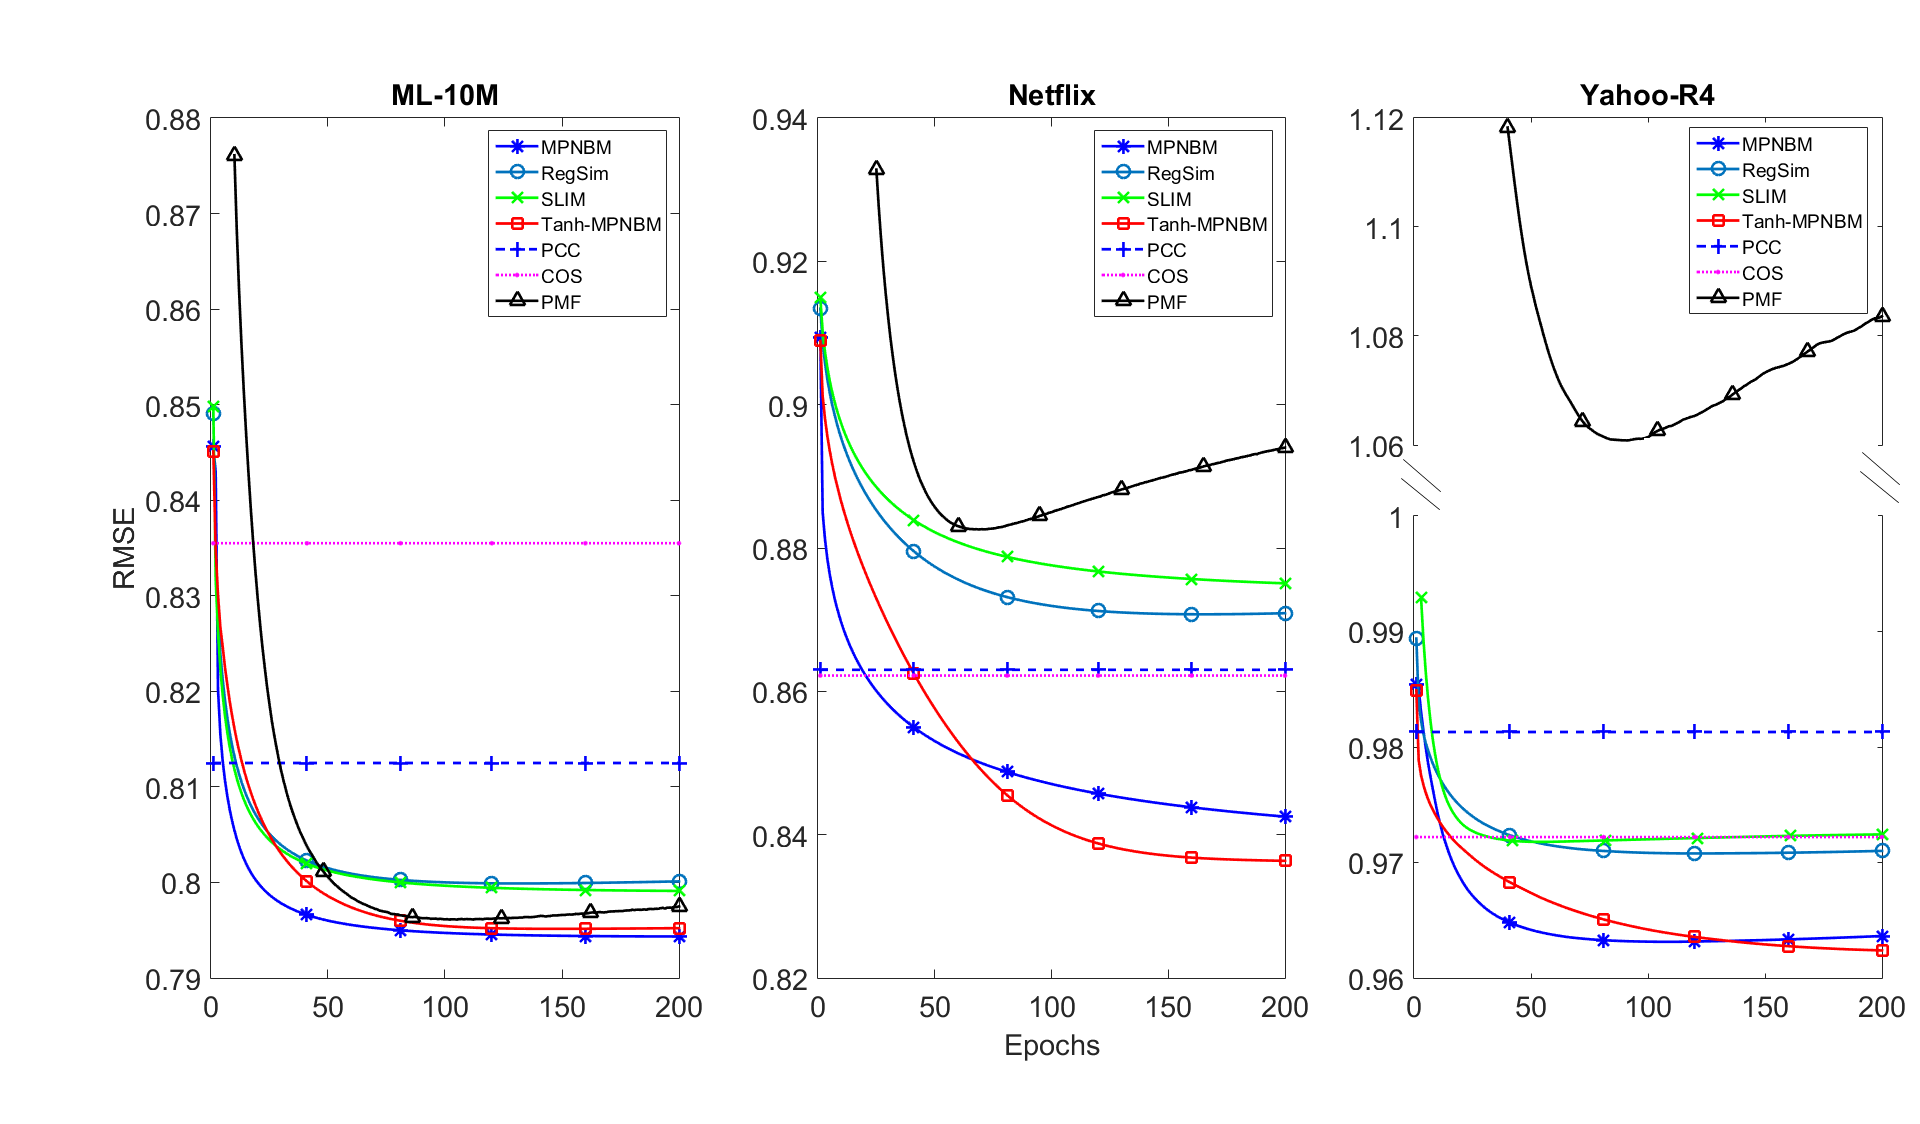
\includegraphics[height=2.8in, width=7in]{expml3-rnm5}
\caption{ RMSE evaluation on ML-10M, Netflix, Yahoo-R4. The Y-axis displays RMSE value and the X-axis shows the number of epochs (iterations) in the training.}
\label{fig:com}
\end{figure*}

\begin{figure*}[!ht]
\hspace*{-0.2cm}
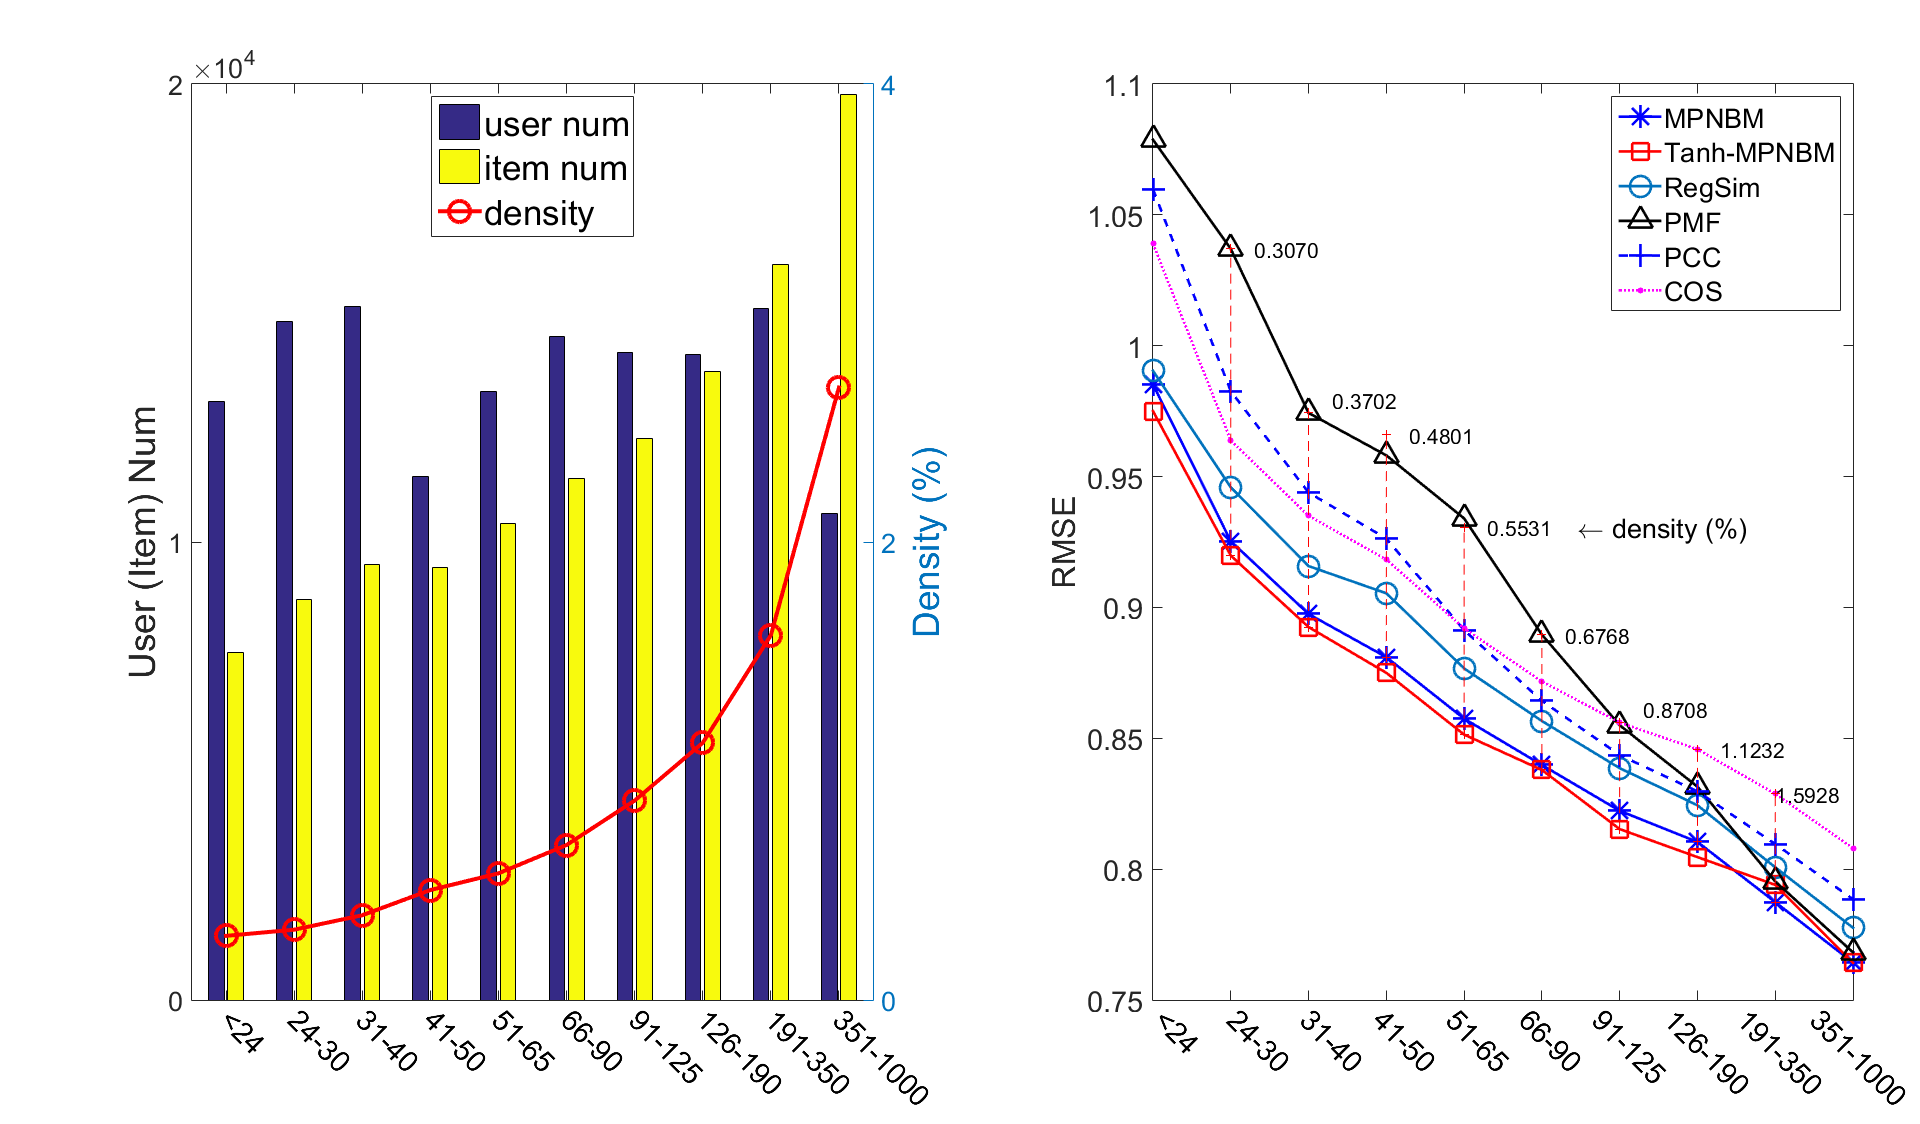
\includegraphics[height=3in, width=6.8in]{diffdensity3}
\caption{ RMSE evaluation with different density. Left panel: Basic information of the 10 subsets extracted from ML-20M. Right panel: The RMSE evaluation on each subset, the Y-axis displays RMSE value. The X-axis of both panels displays the number of rated items per user in each subset.}
\label{diffdensity}
\end{figure*}

\subsection{Models for Comparison}
\label{algfc}
In this paper, the following models are compared:
\begin{itemize}
\item {\bfseries RegSim: } Regression on \emph{similarity}  \cite{toscher2008improved}, a representative work which learns \emph{similarity} via a regression method.
\item {\bfseries SLIM: } Sparse linear methods \cite{ning2011slim}, a regression model for top-$N$ recommendation on binary data set. We extend it to a arbitrary real-value prediction model by placing a jointly Gaussian-Laplace prior on similarity vectors. It has a very similar error function as SLIM,
\begin{equation}
\begin{split}
\mathcal{E}  =   &\frac{1}{2}\sum_{u=1}^{N}\sum_{i=1}^{M} ( r_{ui}-\frac{S_iR_u^-}{|S_i|I_u^-})^{2}I_{ui}  \\
& +\frac{\lambda_S}{2}\sum_{i=1}^{M}||S_{i}||_2-\lambda_S \mu\sum_{i=1}^{M}||S_i||_{1}
 \end{split}
\end{equation}
%\end{tiny}
where $\mu$ is a non-zero mean value of the Gaussian prior.
\item {\bfseries PCC: } NBM using Pearson correlation as \emph{similarity} \cite{resnick1994grouplens}.
\item {\bfseries COS: } NBM using Cosine correlation as \emph{similarity} \cite{desrosiers2011comprehensive}.
\item {\bfseries PMF: } Probabilistic matrix factorization \cite{ruslanpmf}.
\item {\bfseries MPNBM: } In this paper, we exploit influence from ratings as an instance to demonstrate MLSD's ability of modeling various features, thus to improve accuracy. We use a 3-layer \emph{similarity} descriptor in which layer-1 treats latent influence equally with constraint-matrix set to 1; Layer-2 adopts Pearson correlation as constraint-matrix that stresses the influence from those items which either have significant positive correlation or strong negative correlation
with the item under predication; Layer-3 employs Jaccard index to form a constraint-matrix that amplifies the influence from those items which have similar rating history, alleviates the divergence from infrequent-rated items and frequent-rated items. {\bfseries Time Complexity.} The computational time is mainly taken by updating \emph{similarity}. At a single epoch,
approximately $T \cdot \mathcal{L}\cdot \#_u$ similarities are updated, where $\mathcal{L}$ is the size of training set, $\#_u$ is the average rating number per users and $T$ is the number of influence layers. Intuitively, a single epoch takes about 4, 260, 340 seconds on Yahoo-R4, Netflix, ML-10M respectively.
\item {\bfseries Tanh-MPNBM: } The model which we pass MPNBM through hyperbolic tangent function ( detailed in Section \ref{map-1} ).
\end{itemize}


\emph{Experiment setting.} All models are implemented with Matlab, and run on a single core of a Intel (R) Xeon(R) 3.50 GHz machine with 16 GB memory. % The implementation of MPNBM can be found at \footnote{https://github.com/...}.

\subsection{Parameters Setting}
For RegSim, MPNBM, Tanh-MPNBM and SLIM,
%they share the same parameters on all the three data sets respectively.
we empirically choose parameters for each model after a grid search in which $\beta \in \{0.05, 0.1, 0.2, 0.3, 0.4, 0.5\}, \lambda_1=\lambda_2=\lambda_3 \in \{0.01, 0.02, 0.03, 0.04, 0.05, 0.06, 0.1\}$. The finally chosen parameters are summarized in Table \ref{setpara} ($\perp$ indicates a model does not have such a parameter).
\begin{table}[!ht]
\centering
\caption{Parameters Setting for RegSim, MPNBM, Tanh-MPNBM, SLIM.}
\begin{tabular}{|l|c|c|c|}
\hline
           & $\beta$ & $(\lambda_1,\lambda_2,\lambda_3)$ & $(\phi^{(1)},\phi^{(2)},\phi^{(3)})$ \\ \hline
RegSim       & 0.1     & (0.01,$\perp$,$\perp$)           & ($\perp$,$\perp$,$\perp$)                              \\ \hline
MPNBM      & 0.2     & (0.05,0.05,0.05)                 & (3,1,1)                                                \\ \hline
Tanh-MPNBM & 0.4     & (0.05,0.05,0.05)                 & (3,1,1)                                                \\ \hline
SLIM    & 0.4     & (0.02,$\perp$,$\perp$)           & ($\perp$,$\perp$,$\perp$)                              \\ \hline
\end{tabular}

\label{setpara}
\end{table}

For PMF,  we choose latent feature dimension $D=10$ and the momentum of mini-batch SGD $\eta=0.8$. Regularized parameters ($\lambda_P, \lambda_Q$ for user latent factors and latent item factors respectively) and learning rate $\beta$ are set to

\begin{itemize}
\item For Yahoo-R4, $\lambda_P=\lambda_Q=0.05$ and $\beta=0.0005$.
\item For Netflix, $\lambda_P=\lambda_Q=0.002$ and $\beta=0.0002$.
\item For ML-10M, $\lambda_P=\lambda_Q=0.02$ and $\beta=0.0002$.
\item For the first two ML-20M subsets shown in the left panel of Fig. \ref{diffdensity}, $\lambda_P=\lambda_Q=0.01$ and $\beta=0.0002$.
\item For the other eight ML-20M subsets shown in the left panel of Fig. \ref{diffdensity}, $\lambda_P=\lambda_Q=0.02$ and $\beta=0.0002$.
\end{itemize}

For PCC and COS, we use top-200 the most similar neighbors for prediction.

\subsection{Comparison Results}
During the test, we randomly divide each data set into training set (85\%), validation set (5\%) and testing set (10\%). We adopt RMSE for evaluation.
We repeat the experiments 5 times.
\begin{table}[!ht]
\small
\centering
\caption{Accuracy Comparison (The smaller RMSE, the better accuracy for recommendation.). MPNB,  TMPN, denote MPNBM and Tanh-MPNBM respectively. }
\begin{tabular}{|l|c|c|c|c|c|c|}
\hline
\multirow{2}{*}{} & \multicolumn{2}{l|}{Yahoo-R4} & \multicolumn{2}{c|}{Netflix}                & \multicolumn{2}{l|}{ML-10M} \\ \cline{2-7}
                  & RMSE       & INC\%            & RMSE                        & INC\%         & RMSE      & INC\%           \\ \hline
RegSim              & 0.9723     & 0             & 0.8713                      & 0        & 0.8034    & 0           \\ \hline
MPNB             & 0.9641     & \textbf{0.84}    & 0.8425                      & \textbf{3.31} & 0.7941    & \textbf{1.16}   \\ \hline
TMPN      & 0.9629     & \textbf{0.97}    & 0.8363                      & \textbf{4.02} & 0.7955    & \textbf{0.98}   \\ \hline
SLIM           & 0.9725     & -0.02             & 0.8731                      & -0.21         & 0.8004    & 0.37            \\ \hline
PMF               & 1.0608     & -9.1            & 0.8826                      & -1.3         & 0.7957    & 0.96             \\ \hline
PCC               & 0.9813     & -0.93                & \multicolumn{1}{l|}{0.8620} & 1.07             & 0.8121    & -1.08               \\ \hline
COS               & 0.9722     & 0.01             & \multicolumn{1}{l|}{0.8605} &1.24          & 0.8362    & -4.08           \\ \hline
\end{tabular}
\label{accuracy-table-rmse}
\end{table}

\subsubsection{Accuracy}
\label{cpt}
The comparison is performed over :
\begin{itemize}
\item Accuracy on different data sets.
\item Accuracy on different density.
\end{itemize}

Fig. \ref{fig:com}  presents the detail of training on different data sets. Table \ref{accuracy-table-rmse} records the final accuracy  comparison (the training process is conducted by validation set). RegSim is selected as baseline model,  the accuracy improvement of each model is displayed in the INC \% column.
%The improvements by the best model on all the three data sets are statistically significant ($p \text{-} value <0.01$).

Fig. \ref{diffdensity} shows the accuracy comparison on data sets with different density.  MPNBM and Tanh-MPNBM consistently outperform outperform state-of-art models, especially on those extremely sparse data sets ( which have serious \emph{cold start} problem). For simplicity, we don't draw SLIM on the graph, since SLIM has similar accuracy with RegSim.


\begin{figure}[!ht]
\hspace*{-0.4cm}
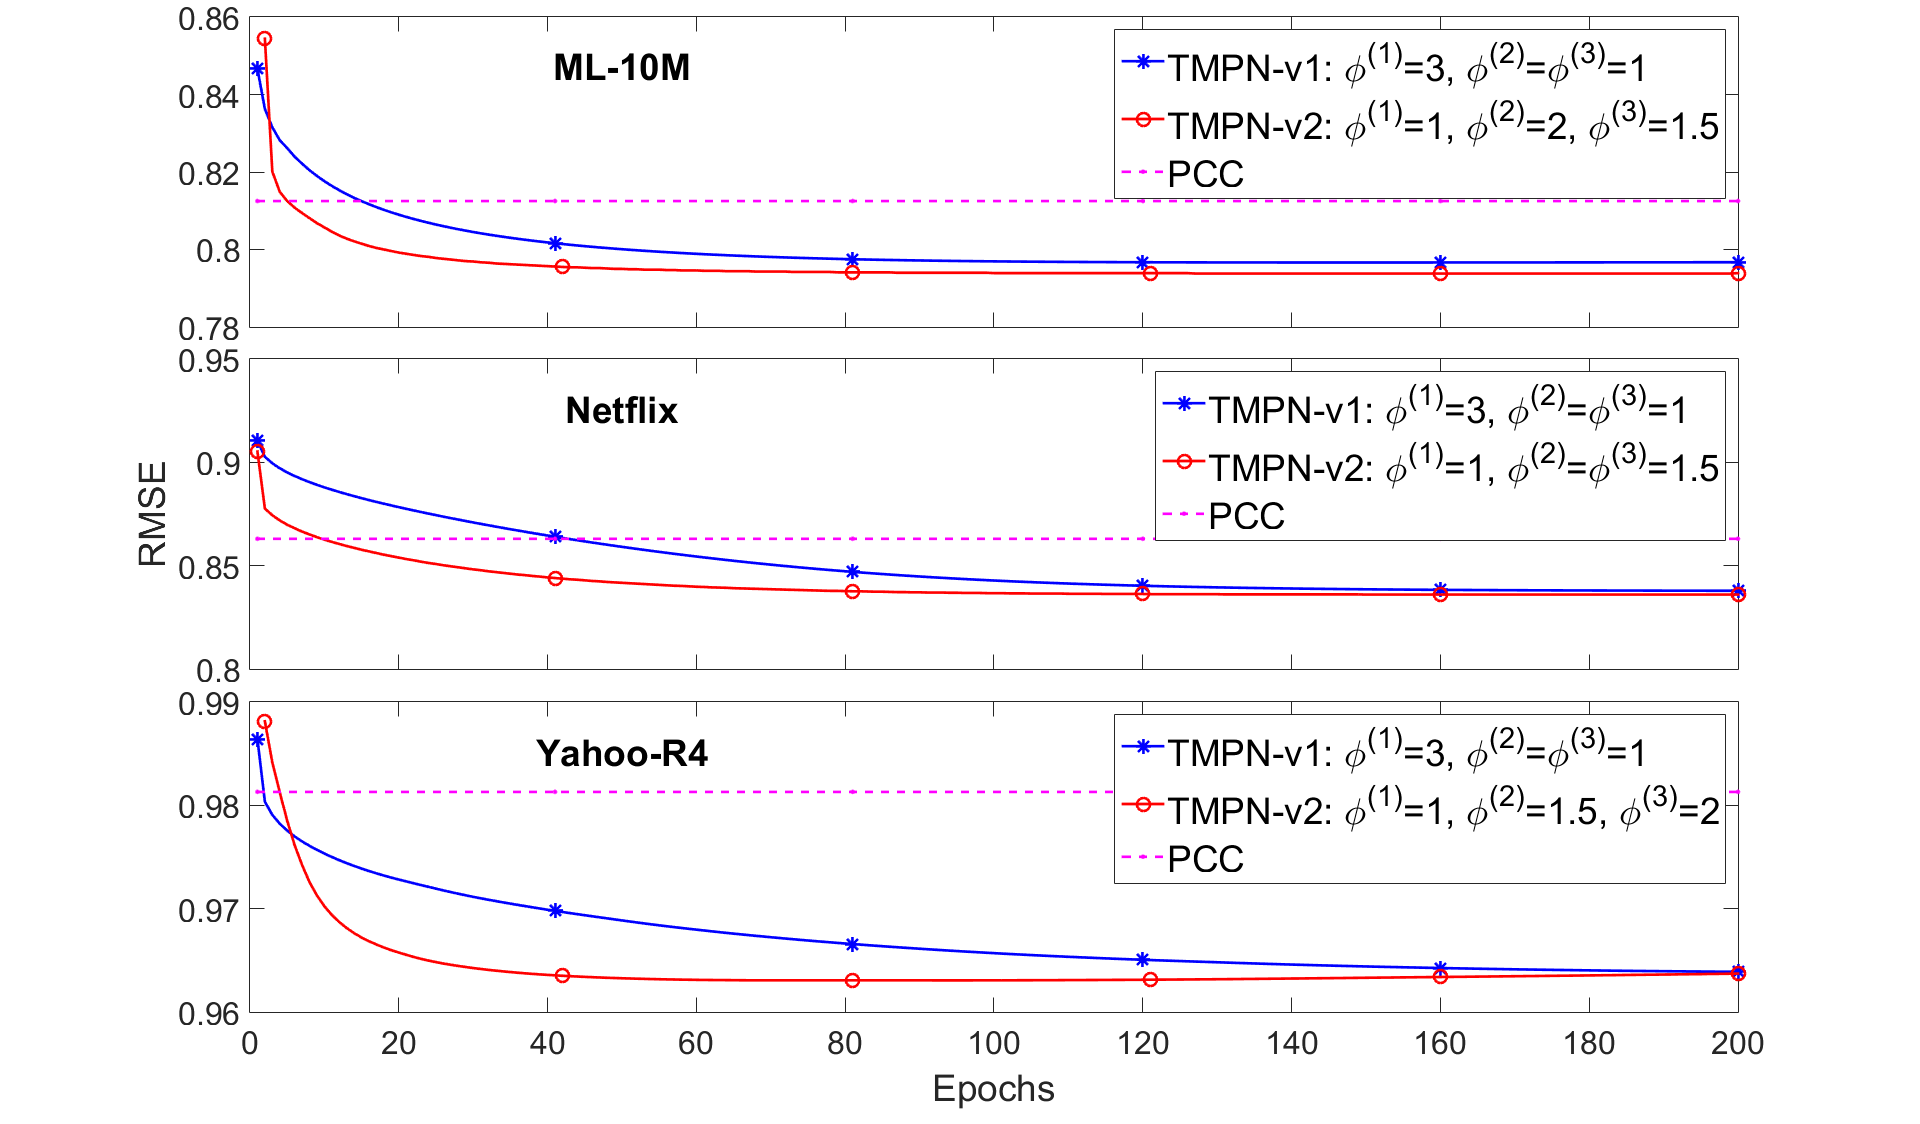
\includegraphics[height=2.8in, width=3.7in]{toyexp5}
\caption{ Tanh-MPNBM: Comparison between two strategies of setting $\phi$. }
\label{fig:toy}
\end{figure}

\vspace{0.2cm}

We are also interested in that how the layer importance-factor $\phi$ affects the MPNBM (Tanh-MPNBM). We use two strategies to select parameters $\phi$ for each layer, 1) we consistently choose $\phi^{(1)}=3,\ \phi^{(2)}=\phi^{(3)}=1$ for all the three data sets, named TMPN-V1; 2) letting $\phi^{(t)} \in \{1, 1.5, 2 \}$, we assign higher value to the $\phi$ which corresponding $\Omega$ has lower RMSE, named TMPN-V2.  The comparison is shown in Fig. \ref{fig:toy}, and 1) the accuracy is not significantly influenced, MPNBM (Tanh-MPNBM) is able to balance the influence automatically. 2) Assigning proper weight to $\phi$ according to the RMSE of $\Omega$ results in faster convergence.

\subsubsection{Stability}

Model based approach may easily over fit when increasing the number of parameters under training. The system can be beneficent from the stability of algorithms which is defined by
\begin{itemize}
\item converge speed: the first epoch where a model converges to the local best solution, denoted as $\epsilon$.
\item  ability of models to maintain their best status: the number of epochs that a model stays in the local best solution, denoted as $\zeta$.
\end{itemize}

Table \ref{stable-table} shows the values of $\epsilon$ and $\zeta$ of each model over different data sets.
\begin{table}[h!]
\centering
\caption{Stability Comparison}
\begin{tabular}{|l|c|c|c|c|c|c|}
\hline
\multirow{2}{*}{} & \multicolumn{2}{l|}{Yahoo-R4} & \multicolumn{2}{c|}{Netflix} & \multicolumn{2}{l|}{ML-10M} \\ \cline{2-7}
                  &     $\epsilon$          &    $\zeta $           &              $\epsilon$  &      $\zeta $         &     $\epsilon$           &            $\zeta $  \\ \hline
RegSim              & 86            & 102           & 134           & $\geq$67           & 96            & 91          \\ \hline
MPNBM             & 84            & 59            & \multicolumn{2}{c|}{*}       & 141           & $\geq$60          \\ \hline
Tanh-MPNBM        & 158           & $\geq$43            & 166           & $\geq$35           & 115           & $\geq$86          \\ \hline
SLIM           & 39             & 51             & 186             & $\geq$15            & 150             & $\geq$51           \\ \hline
PMF               & 87            & 6             & 64            & 12           & 93            & 34          \\ \hline
\end{tabular}
\label{stable-table}
\end{table}
In the comparison of stability, we treat RMSE values $x_1 = x_2$, if $|x_1-x_2|\leq 0.0001$. Note that with regard to a model which does not over fit after 200 epochs (value of $\zeta$ prefixed with $\geq$), if the lowest RMSE value appears at least 10 epochs, it is seen as the local best solution. * in Table \ref{stable-table} means a model does not converge after 200 epochs on a data set. e.g, MPNBM does not converge on Netflix data set, also shown in Fig. \ref{fig:com}. The experimental results show that MPNBM and Tanh-MPNBM stay in the local best solution for many ( $>$ 40) epochs which is better than PMF. With regard to converge speed, as shown in Table \ref{stable-table}, it seems that sometimes MPNBM and Tanh-MPNBM do not converge as fast as PMF. In fact, they achieve a considerable accuracy at a much earlier epoch.

\section{Conclusion}
\label{conclusion}
In this paper, we have presented a probabilistic framework of NBM family, and introduced a multi-layer \emph{similarity} descriptor under PNBM which is capable of modeling and learning the joint influence of various features. Our experiments show that MPNBM and Tanh-MPNBM allow accurate and stable estimation of user preferences.

Privacy is a serious problem to recommender systems. Nowadays, applying differential privacy to recommendation algorithms attracts great attention. A common approach is adding noise to data set. Recently, people find that sampling from a posterior distribution achieves some extent of differential privacy ``for free" \cite{wang2015privacy}, and this idea has been already successfully applied to probabilistic matrix factorization \cite{liu2015fast}. Following the same idea, our models can also provide such kind of ``free privacy". We leave a detailed investigation as future work.

\section{Acknowledgments}
Both authors are supported by a CORE (junior track) grant from the National Research Fund, Luxembourg. Qiang Tang is also partially supported by an internal project from University of Luxembourg.

%
% The following two commands are all you need in the
% initial runs of your .tex file to
% produce the bibliography for the citations in your paper.
\bibliographystyle{abbrv}
\bibliography{sigproc}  % sigproc.bib is the name of the Bibliography in this case

% that's all folks
\end{document}


